\documentclass[12pt, a4paper]{article}

\usepackage[margin=1in]{geometry}
\usepackage{booktabs}
\usepackage{listings}
\usepackage{xcolor}
\usepackage{tikz}
\usepackage{pgfplots}
\pgfplotsset{compat=1.18}
\usepackage{float}
\usepackage{parskip}

% simple code style
\lstset{
    basicstyle=\ttfamily\small,
    backgroundcolor=\color{gray!10},
    frame=single,
    breaklines=true,
    numbers=left,
    numberstyle=\tiny\color{gray},
    showstringspaces=false,
}

\begin{document}

% ── Title ─────────────────────────────────────────────────────
\begin{center}
    {\Large \textbf{Lab 5 — Lexical Analysis}}\\[0.5em]
    {\large 2023-CS-18 M Ahmed}\\[0.3em]
    \today
\end{center}

\bigskip
\hrule
\bigskip

% ── 1. What we did ────────────────────────────────────────────
\section*{1. Overview}

In this lab we built a lexical analyzer for a subset of Pascal
(from Dragon Book Appendix A). The job of a lexical analyzer is to
read source code and break it into tokens — things like keywords,
identifiers, numbers, and operators.

We implemented the same lexer three different ways so we could
compare how each approach works and how fast each one runs.

% ── 2. The Language ───────────────────────────────────────────
\section*{2. Pascal Subset Tokens}

The grammar gives us these token types:

\begin{center}
\begin{tabular}{lll}
\toprule
Token & What it matches & Example \\
\midrule
KEYWORD   & reserved words                  & \texttt{begin, if, while} \\
ID        & letter followed by letters/digits & \texttt{gcd, x, myVar} \\
NUM       & integer or real number           & \texttt{42, 3.14, 1.5E10} \\
ASSIGNOP  & assignment                       & \texttt{:=} \\
RELOP     & comparison                       & \texttt{=, <>, <, <=, >, >=} \\
ADDOP     & addition level                   & \texttt{+, -, or} \\
MULOP     & multiplication level             & \texttt{*, /, div, mod, and} \\
DOTDOT    & array range                      & \texttt{..} \\
\bottomrule
\end{tabular}
\end{center}

Comments are written inside \texttt{\{ \}} and cannot be nested.
Whitespace is ignored everywhere.

% ── 3. Approach 1 ─────────────────────────────────────────────
\section*{3. Approach 1 — State-Based DFA}

This approach uses one loop and one \texttt{state} variable.
Every character we read moves us to a new state. When the state
tells us a token is complete, we return it.

For example: reading \texttt{:} moves us to state \texttt{COLON}.
Then if the next character is \texttt{=} we return \texttt{ASSIGNOP :=},
otherwise we return \texttt{COLON :}.

The states we used are:

\begin{center}
\begin{tabular}{ll}
\toprule
State & Meaning \\
\midrule
START     & waiting for first character \\
ID        & reading an identifier \\
INT       & reading integer digits \\
FRAC      & reading decimal part \\
EXP       & reading exponent \\
COLON     & saw \texttt{:}, waiting to see if next is \texttt{=} \\
LT        & saw \texttt{<}, waiting for \texttt{=} or \texttt{>} \\
GT        & saw \texttt{>}, waiting for \texttt{=} \\
DOT       & saw \texttt{.}, waiting for second \texttt{.} \\
\bottomrule
\end{tabular}
\end{center}

% ── 4. Approach 2 ─────────────────────────────────────────────
\section*{4. Approach 2 — Stateless}

This approach has no state variable at all. Instead,
\texttt{next\_token()} just looks at the first character and
immediately calls the right helper function.

If it sees a letter it calls \texttt{scan\_word()}.
If it sees a digit it calls \texttt{scan\_num()}.
If it sees \texttt{:} it handles it inline.
Each case is completely independent of the others.

This is the simplest approach to read and understand.
Adding a new token type just means adding one new \texttt{if} line.

% ── 5. Approach 3 ─────────────────────────────────────────────
\section*{5. Approach 3 — Transition Table}

This approach puts all the DFA transitions into a 2D table:

\[
\texttt{table[current\_state][char\_class] = next\_state}
\]

Every character is first classified into a class (like
\texttt{DIGIT}, \texttt{LETTER}, \texttt{EQ}, etc.).
Then we just look up the table to find the next state.
The loop itself has no \texttt{if/elif} logic for token types at all.

This is how real tools like \texttt{lex} and \texttt{flex} work.
The advantage is that you can change the language just by changing
the table — the driver loop stays the same.

\subsection*{Bonus — Compressed Table}

The full table has $12 \times 22 = 264$ cells but only 58 of them
are not error entries. So we also built a compressed version that
stores only the 58 useful entries in a dictionary.
This saves 78\% of the memory with almost no speed difference.

% ── 6. Sample Output ──────────────────────────────────────────
\section*{6. Sample Output}

We tested all approaches on the GCD program from Figure A.1 in
the Dragon Book. All four produced exactly the same 68 tokens.
Here are the first few lines:

\begin{lstlisting}[language={}]
  Line  Type         Lexeme           Value
  -----------------------------------------------
  1     KEYWORD      program          -
  1     ID           example          -
  1     LPAREN       (                -
  1     ID           input            -
  1     COMMA        ,                -
  1     ID           output           -
  1     RPAREN       )                -
  1     SEMICOLON    ;                -
  2     KEYWORD      var              -
  2     ID           x                -
  ...
  Total: 68 tokens
\end{lstlisting}

% ── 7. Speed Results ──────────────────────────────────────────
\section*{7. Speed Comparison}

We ran each lexer 1000 times on a 10,040 character source file
(3,021 tokens) and measured the average time per run.

\begin{center}
\begin{tabular}{clrr}
\toprule
Rank & Approach & Time (ms) & vs Fastest \\
\midrule
1 & Approach 2 — Stateless        & 0.1455 & 1.00x \\
2 & Approach 1 — State-Based DFA  & 0.1646 & 1.13x \\
3 & Approach 3 — Transition Table & 0.3033 & 2.08x \\
4 & Bonus — Compressed Table      & 0.3241 & 2.23x \\
\bottomrule
\end{tabular}
\end{center}

\begin{figure}[H]
\centering
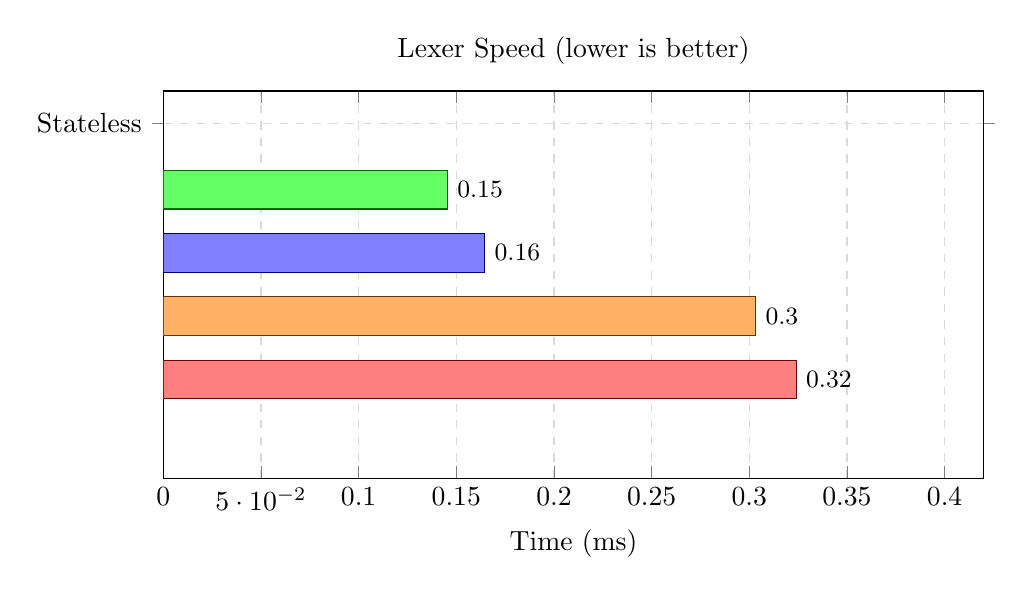
\begin{tikzpicture}
\begin{axis}[
    xbar,
    width=12cm,
    height=6.5cm,
    bar width=14pt,
    xlabel={Time (ms)},
    symbolic y coords={
        {Compressed Table},
        {Transition Table},
        {State-Based DFA},
        {Stateless}
    },
    ytick=data,
    xmin=0, xmax=0.42,
    nodes near coords,
    nodes near coords style={font=\small},
    grid=major,
    grid style={dashed, gray!30},
    title={Lexer Speed (lower is better)},
]
\addplot[fill=green!60, draw=green!40!black]
    coordinates {(0.1455,{Stateless})};
\addplot[fill=blue!50, draw=blue!40!black]
    coordinates {(0.1646,{State-Based DFA})};
\addplot[fill=orange!60, draw=orange!40!black]
    coordinates {(0.3033,{Transition Table})};
\addplot[fill=red!50, draw=red!40!black]
    coordinates {(0.3241,{Compressed Table})};
\end{axis}
\end{tikzpicture}
\caption{Average time per run for each approach (1000 runs)}
\end{figure}

\textbf{Why Approach 2 is fastest:} It uses plain \texttt{if} checks
on one character with no extra overhead. Approach 3 is slower because
every character needs two extra steps — classify it into a class, then
do a table lookup. The compressed table is slightly slower than the
full table because dictionary lookup is a bit slower than a direct
list index.

% ── 8. Summary ────────────────────────────────────────────────
\section*{8. Summary}

\begin{center}
\begin{tabular}{lccc}
\toprule
 & Approach 1 & Approach 2 & Approach 3 \\
\midrule
Speed       & Fast    & Fastest & Slow \\
Easy to read & Medium & Yes     & No  \\
Easy to change & Medium & Yes   & Yes (edit table) \\
Auto-generate & No    & No      & Yes \\
\bottomrule
\end{tabular}
\end{center}

Approach 2 is the best choice if you are writing a lexer by hand.
Approach 3 is the right choice when using a tool that generates the
lexer automatically from grammar rules.
\subsection{Screenshot of Execution Approach 1}
\begin{center}
\includegraphics[width=0.8\textwidth]{s1.png}
\end{center}
\begin{center}
\includegraphics[width=0.8\textwidth]{s2.png}
\end{center}
\subsection{Screenshot of Execution Approach 2}
\begin{center}
\includegraphics[width=0.8\textwidth]{s3.png}
\end{center}
\subsection{Screenshot of Execution Approach 3}
\begin{center}
\includegraphics[width=0.8\textwidth]{s4.png}
\end{center}
\subsection{Screenshot of Execution Approach 4}
\begin{center}
\includegraphics[width=0.8\textwidth]{s5.png}
\end{center}
\subsection{Comparision}
\begin{center}
\includegraphics[width=0.8\textwidth]{Screenshot 2026-03-16 151639.png}
\end{center}
\end{document}